\documentclass[conference]{IEEEtran}

\usepackage{iftex}
\ifXeTeX
  % Tectonic/XeTeX: use a Times clone so the output matches IEEE's pdfTeX look.
  \usepackage{fontspec}
  % Load by file name: Tectonic has no fontconfig, so family names do not resolve.
  \setmainfont{texgyretermes}[Extension=.otf, UprightFont=*-regular, BoldFont=*-bold,
    ItalicFont=*-italic, BoldItalicFont=*-bolditalic]
  \setsansfont{texgyreheros}[Extension=.otf, UprightFont=*-regular, BoldFont=*-bold,
    ItalicFont=*-italic, BoldItalicFont=*-bolditalic]
  \setmonofont{texgyrecursor}[Extension=.otf, UprightFont=*-regular, BoldFont=*-bold,
    ItalicFont=*-italic, BoldItalicFont=*-bolditalic]
\else
  \usepackage[T1]{fontenc}
  \usepackage{newtxtext,newtxmath}
\fi
\usepackage{cite}
\usepackage{amsmath,amssymb}
\usepackage{graphicx}
\usepackage{booktabs}
\usepackage{siunitx}
\usepackage{xcolor}
\usepackage[hidelinks]{hyperref}

\graphicspath{{figures/}}

\begin{document}

\title{A Vision-Guided, AI-Supervised Robotic Sorting Cell on an IEC 61131-3 Soft-PLC with a MuJoCo Digital Twin}

% TODO(P7): real author metadata from owner (names, department, university, city, email).
\author{\IEEEauthorblockN{Author Name}
\IEEEauthorblockA{\textit{Department} \\
\textit{University}\\
City, Country \\
email@example.com}}

\maketitle

\begin{abstract}
% TODO(P7): 150--250 words. Problem, architecture (PLC / vision / decision layer / twin),
% key quantitative results from experiments/results/, conclusion.
This paper presents a vision-guided robotic sorting and quality-inspection cell.
\end{abstract}

\begin{IEEEkeywords}
IEC 61131-3, CODESYS, robot control, PackML, computer vision, open-vocabulary detection,
decision model, digital twin, OPC UA, HMI
\end{IEEEkeywords}

\section{Introduction}\label{sec:introduction}
% TODO(P7): motivation (flexible sorting, quality inspection on PLC-based cells).
% TODO(P7): gap: AI perception and decisions rarely integrated with IEC 61131-3 control \cite{IEC61131-3}.
% TODO(P7): contributions list (architecture, open implementation, measured evaluation).

Placeholder: this section will be written in a later phase~\cite{IEC61131-3}.

\section{Related Work}\label{sec:related-work}
% TODO(P7): vision-language-action models (Helix-02, OpenVLA, pi0) and why they are not used.
% TODO(P7): world models (V-JEPA 2); decision models (THX-02 \cite{HALX2026thx02}).
% TODO(P7): open-vocabulary detection (YOLOE \cite{Wang2025yoloe}, YOLOE-26 \cite{Sapkota2026yoloe26}).

Placeholder: this section will be written in a later phase~\cite{HALX2026thx02}~\cite{Wang2025yoloe}~\cite{Sapkota2026yoloe26}.

\section{System Architecture}\label{sec:architecture}

The cell sorts three part types arriving on a moving conveyor into six bins: one bin per good
type (Type~A, B, C) plus Rework, Scrap and Quarantine. A 6-axis articulated arm with a suction
gripper picks each part from the moving belt. There is no hardware: the plant is a MuJoCo
digital twin (Section~\ref{sec:twin}), and the controller is a CODESYS soft-PLC running an
IEC~61131-3 application~\cite{IEC61131-3}.

\subsection{Layers and Real-Time Boundaries}

The system is split into layers with different time scales (Fig.~\ref{fig:architecture}). One
rule connects them: a slower layer never blocks a faster one. The PLC never waits for vision or
for the decision layer. If a vision result is missing, the part is not picked; if a decision is
late, the PLC applies its own rule.

\begin{figure}[t]
\centering
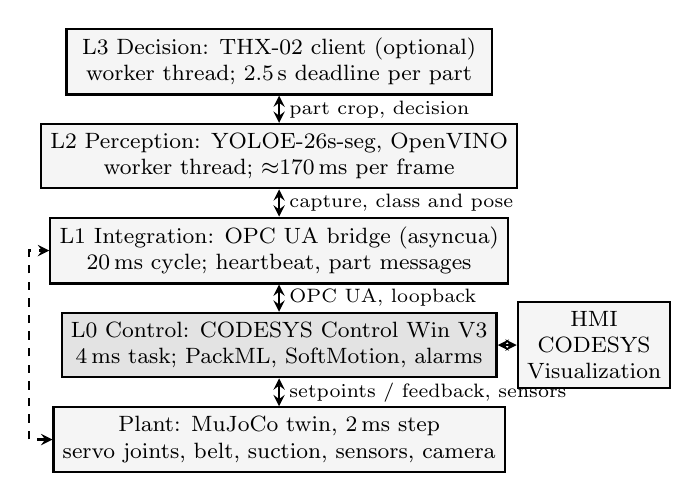
\begin{tikzpicture}[
    font=\footnotesize,
    layer/.style={draw, thick, rectangle, minimum width=5.4cm, minimum height=0.8cm,
                  align=center, fill=gray!8},
    plc/.style={layer, fill=gray!22},
    side/.style={draw, thick, rectangle, minimum width=1.5cm, minimum height=0.85cm,
                 align=center, fill=gray!8},
    arr/.style={<->, >=stealth, thick}]
  \node[layer] (l3) at (0,4.8) {L3 Decision: THX-02 client (optional)\\worker thread; 2.5\,s deadline per part};
  \node[layer] (l2) at (0,3.6) {L2 Perception: YOLOE-26s-seg, OpenVINO\\worker thread; $\approx$170\,ms per frame};
  \node[layer] (l1) at (0,2.4) {L1 Integration: OPC UA bridge (asyncua)\\20\,ms cycle; heartbeat, part messages};
  \node[plc]   (l0) at (0,1.2) {L0 Control: CODESYS Control Win V3\\4\,ms task; PackML, SoftMotion, alarms};
  \node[layer] (pl) at (0,0.0) {Plant: MuJoCo twin, 2\,ms step\\servo joints, belt, suction, sensors, camera};
  \node[side]  (hmi) at (4.0,1.2) {HMI\\CODESYS\\Visualization};
  \draw[arr] (l3) -- node[right, font=\scriptsize] {part crop, decision} (l2);
  \draw[arr] (l2) -- node[right, font=\scriptsize] {capture, class and pose} (l1);
  \draw[arr] (l1) -- node[right, font=\scriptsize] {OPC UA, loopback} (l0);
  \draw[arr] (l0) -- node[right, font=\scriptsize] {setpoints / feedback, sensors} (pl);
  \draw[arr] (l0) -- (hmi);
  \draw[<->, >=stealth, thick, dashed] (pl.west) -- ++(-0.3,0) |- (l1.west);
\end{tikzpicture}
\caption{Control layers of the cell. The PLC (L0) is master of motion; the twin is master of
physical objects. Solid arrows show the logical data flow. The bridge and the twin run in one
Python process, so the PLC's exchange with the twin passes through the 20\,ms bridge cycle
(dashed).}
\label{fig:architecture}
\end{figure}

\subsection{Who Is Master of What}

Joint setpoints, the tool centre point (TCP) pose and the conveyor position are owned by the PLC:
the robot axes and the conveyor are SoftMotion virtual drives that generate setpoints. The twin
does not copy them. Each joint is a simulated servo drive that tracks the setpoint and reports
its measured position and torque back. The 20\,ms OPC UA link cannot close a servo loop, so the
servo loop lives in the twin, as it would in a real drive, and the PLC does trajectory generation
and supervision. Physical objects (parts on the belt, in the gripper, in the bins) are owned by
the twin; the PLC learns their state only through simulated sensors (photo-eyes, vacuum switch,
bin-full signals, door, E-stop). Class and pose come from vision and, optionally, quality from the
decision layer; once written into the PLC's part record, the PLC owns them.

\subsection{Life of a Part}

The twin spawns a part upstream. When the part interrupts photo-eye PE1, the PLC latches the belt
position, assigns a part id and publishes a capture request. The vision worker renders the camera
image and returns the part's class, confidence and pose $(x, y, \theta)$ in the belt frame at the
capture. If a decision service is configured, it adds a quality disposition and an
identification-reliability answer. The PLC selects the bin, waits until the part is inside the
pick window, tracks it with the robot, picks it with suction and places it in the bin.

\subsection{PLC--Python Interface}

The PLC and the Python services exchange data over OPC UA~\cite{IEC62541}. The CODESYS OPC UA
server publishes only two global variable lists: \texttt{GVL\_Bridge} (setpoints, feedback,
sensors, part messages, diagnostics) and \texttt{GVL\_Hmi} (operator commands). Tag names have a
single source of truth, \texttt{config/opcua\_tags.yaml}. Every message structure carries a
sequence number that the bridge writes last and that the PLC uses to accept each message exactly
once (\texttt{FB\_MessageIntake}). The bridge toggles a heartbeat every cycle; if the PLC sees no
change for 500\,ms it raises a critical alarm and the cell aborts. The endpoint is anonymous and
unencrypted but bound to the loopback interface, with the runtime's inbound firewall rules
disabled. This is acceptable only for a single-host laboratory cell; a plant would use signed and
encrypted sessions.

\section{PLC Control}\label{sec:plc}
% TODO(P1): task configuration, OOP program organisation, PackML states and modes \cite{ISA-TR88.00.02}.
% TODO(P1): SoftMotion axis group, 6-DOF kinematics, conveyor tracking.
% TODO(P1): alarms, interlocks, joint supervision.

Placeholder: this section will be written in a later phase~\cite{ISA-TR88.00.02}.

\section{Perception}\label{sec:perception}
% TODO(P3): camera model and calibration, zero-shot detection with YOLO26 \cite{Ultralytics2026yolo26}.
% TODO(P3): pose estimation from masks, OpenVINO deployment.

Placeholder: this section will be written in a later phase~\cite{Ultralytics2026yolo26}.

\section{AI Decision Layer}\label{sec:decision}

\subsection{Role}

The optional decision layer adds a quality judgement to the detector's class label. It uses
THX-02~\cite{HALX2026thx02}, a decision model that answers typed questions over text and images
with probabilities, through its hosted API. The layer never commands motion: it only fills
decision fields of a part record, and the PLC acts on them inside its own interlocks and
bin-selection rule (Section~\ref{sec:plc}). The PLC does not depend on it: with
the layer switched off, \texttt{GVL\_Bridge.xDecisionActive} is FALSE and the PLC decides each
part by its rule as soon as vision has identified it.

\subsection{Questions and Bin Selection}

One request per part carries the part's image crop, the detected class and confidence, and two
questions: a \emph{choice} between \texttt{ok}, \texttt{rework} and \texttt{scrap} (each defined by a
short criterion), and a yes/no question whether the identification is reliable. The client maps
the answers to \texttt{ST\_DecisionMsg}: the chosen quality with its probability, and
\emph{unreliable} when the probability of ``no'' is at least 0.8. In \texttt{F\_SelectBin} an
unreliable identification sends the part to Quarantine, Scrap and Rework go to their bins, and
only parts judged \texttt{ok} reach their type bin. The detector's class and the decision both
change where the robot places the part.

\subsection{Timing, Rate Limit and Fallback}

The decision for a part must arrive within the PLC's deadline of 2.5\,s after the capture; the
client's time budget is that deadline minus the time already spent. Requests run in a worker
thread with its own event loop, and the bridge polls the answers once per 20\,ms cycle, so a slow
or stalled API cannot delay the cycle. The free tier of the API counts every question, so a part
costs two decisions; a client-side token bucket allows 50 decisions per minute (burst~2), i.e.\
25 parts per minute, below the 60 per minute per address that the API allows. A request that
would exceed the deadline, a rate-limit answer (HTTP~429) that asks for more than 1\,s of waiting,
or any other error ends in the fallback. Fallback decisions are never written to the PLC: the
part keeps waiting until the PLC's own deadline passes and is then decided by the rule, with a
\emph{DecisionFallback} warning on the HMI. A decision that arrives after its part has reached
the pick window is dropped.

\subsection{Record and Replay}

Every exchange is written to a JSON-lines file (run id, seed, part id, time stamp, latency,
request hash, response or fallback reason). A replay mode feeds a recording back into a run, so
results can be recomputed without the API, whose hosted model is not version-pinned.

\subsection{Status}

The decision layer, its rate limiter, deadline handling and record/replay are implemented and
covered by unit tests with a mocked HTTP API, and the request format was checked with one call
using a synthetic image. The layer was \emph{not} used in any of the cell runs reported in
Section~\ref{sec:evaluation}; in those runs the PLC decided every part by its rule. The twin
also does not yet generate defective parts, so the quality decision has no ground truth, and the
planned comparison of the rule baseline with the decision layer is future work. The alarm-triage
advice in the original design was not implemented.

\section{Digital Twin}\label{sec:twin}
% TODO(P2): MuJoCo scene \cite{Todorov2012mujoco}, simulated servo joints, suction gripper, sensors.
% TODO(P2): scenario configuration and fault injection.

Placeholder: this section will be written in a later phase~\cite{Todorov2012mujoco}.

\section{Operator Interface}\label{sec:hmi}
% TODO(P5): ISA-101 high-performance design principles \cite{ISA-101.01}, screen hierarchy.
% TODO(P5): alarm presentation \cite{ISA-18.2}, user roles.

Placeholder: this section will be written in a later phase~\cite{ISA-101.01}~\cite{ISA-18.2}.

\section{Evaluation}\label{sec:evaluation}
% TODO(P6): setup, KPIs, results tables/figures generated from experiments/results/.
% TODO(P6): ablation rule-based vs. YOLO+THX-02; fault-injection results; limitations.

Placeholder: this section will be written in a later phase.

\section{Conclusion}\label{sec:conclusion}
% TODO(P7): summary of results, limitations (soft real-time, hosted API), future work.

Placeholder: this section will be written in a later phase.


\bibliographystyle{IEEEtran}
\bibliography{references}

\end{document}
